\documentclass[t]{beamer}
\usetheme{Boadilla}

\usepackage{animate}
\usepackage[english]{babel}
\usepackage[font=tiny]{caption}
\usepackage[outputdir=/home/wlt/.cache/gummi/]{minted}
\usepackage{multicol}
\usepackage{multirow}
\usepackage{setspace}
\usepackage{tikz}

\usetikzlibrary{automata, positioning, arrows, babel, positioning, shapes}

\newcommand{\eg}{\textit{e}.\textit{g}., }
\newcommand{\ie}{\textit{i}.\textit{e}., }
\newcommand{\heading}[1]{{\it{\usebeamercolor[fg]{frametitle} #1}}}

\definecolor{osprey_blue}{cmyk}{1, .76, .1, .65}
\definecolor{osprey_gray}{cmyk}{.36, .29, .28, 0}
\definecolor{osprey_green}{cmyk}{.59, .02, 1, 0}

\setbeamercolor*{palette primary}{bg=osprey_blue, fg = white}
\setbeamercolor*{palette secondary}{bg=osprey_gray, fg = white}
\setbeamercolor*{palette tertiary}{bg=osprey_blue, fg = white}
\setbeamercolor{structure}{fg=osprey_blue} % itemize, enumerate, etc
\setbeamercolor{section in toc}{fg=osprey_blue} % TOC sections

\setbeamerfont{section in toc}{size=\footnotesize}
\setbeamerfont{subsection in toc}{size=\scriptsize}
\setbeamerfont{subsubsection in toc}{size=\scriptsize}

\setbeamertemplate{enumerate item}[default]
\setbeamertemplate{itemize/enumerate body begin}{\small}
\setbeamertemplate{itemize/enumerate subbody begin}{\tiny}
\setbeamertemplate{itemize/enumerate subsubbody begin}{\tiny}

\setbeamerfont{description body}{size=\small}

\setminted{linenos, escapeinside=@@, fontsize=\footnotesize, tabsize=4, xleftmargin=1cm}
\usemintedstyle{emacs}

\tikzset{declare function={f(\x)=0.25*(\x-2.5)^3-0.75*\x+5);}}


\title[Serial vs. Parallel Implementation]{Serial vs. Parallel Implementation of \\
                                           Definite Integrals using the Trapezoid Rule}
\subtitle{\vspace{1em}\footnotesize Presented by:\vspace{-2em}}
\author[\textbf{Group X}]{\textbf{Group X} \\
                          \footnotesize \textit{Jason Gardner, Matthew Thomas, \& William L Thomson Jr}}
\institute[UNF]{University of North Florida \\
                Parallel Computing COP6616 \\
                Instructor Scott Piersall}
\date{\today}

\begin{document}

\begin{frame}[plain]
	\titlepage
\end{frame}

\begin{frame}[allowframebreaks]{Outline}
	\tableofcontents
	\vfill
\end{frame}

\section{Integration}

\begin{frame}{Area Under The Curve}
\begin{multicols}{2}

\begin{tikzpicture}[line join=round,line cap=round]
	\begin{scope}
	\draw[-latex] (-0.5,0) -- (5,0) node[below] {$x$};
	\draw[-latex] (0,-0.5) -- (0,5) node[left]  {$y$};
	\node at (2,3.5) {$f(x)=0.1 x^2+2$};
    \foreach\i in {1, 2, 3, 4}
        \node at (\i, -0.25){\i};
    \node at (1, -0.7) {$a$};
    \node at (4, -0.7) {$b$};

	\end{scope}

    \fill [osprey_green, domain=1:4, variable=\x]
      (1, 0)
      -- plot ({\x}, {0.1*\x*\x+2})
      -- (4, 0)
      -- cycle;
      
\draw [thick,cyan]
      plot [domain=0:5, variable=\x] ({\x}, {0.1*\x*\x+2}) node[right] at (1.5,2)
      {};

      
	\end{tikzpicture}

\vfill\null
\columnbreak

\begin{itemize}
\item In calculus, definite integrals calculate the area "under the curve".
\pause
\item Suppose $F(x)$ is the anti-derivative of $f(x)$. That is,

\[F(x)= \int f(x) dx\]
\pause
Then, the area under $f(x)$, between $a$ and $b$, is given by the definite integral:

\[\int_a^b f(x) dx = F(b) - F(a).\]
\end{itemize}
\end{multicols}
\end{frame}


\begin{frame}{Area Under The Curve Example}
\begin{multicols}{2}

\begin{tikzpicture}[line join=round,line cap=round]
	\begin{scope}
	\draw[-latex] (-0.5,0) -- (5,0) node[below] {$x$};
	\draw[-latex] (0,-0.5) -- (0,5) node[left]  {$y$};
	\node at (2,3.5) {$f(x)=0.1*x^2+2$};
    \foreach\i in {1, 2, 3, 4}
        \node at (\i, -0.25){\i};
    \node at (1, -0.7) {$a$};
    \node at (4, -0.7) {$b$};

	\end{scope}

    \fill [osprey_green, domain=1:4, variable=\x]
      (1, 0)
      -- plot ({\x}, {0.1*\x*\x+2})
      -- (4, 0)
      -- cycle;
      
\draw [thick,cyan]
      plot [domain=0:5, variable=\x] ({\x}, {0.1*\x*\x+2}) node[right] at (1.5,2)
      {};

      
	\end{tikzpicture}

\vfill\null
\columnbreak

\begin{itemize}
\item The anti-derivative for this example is easy to find:

\[F(x)=\int (\frac{1}{10} x^2 +2) dx\]
\pause
\[= \frac{1}{30} x^3 +2x +C \]
\end{itemize}
\end{multicols}
\end{frame}

\begin{frame}{Area Under The Curve Example}
\begin{multicols}{2}

\begin{tikzpicture}[line join=round,line cap=round]
	\begin{scope}
	\draw[-latex] (-0.5,0) -- (5,0) node[below] {$x$};
	\draw[-latex] (0,-0.5) -- (0,5) node[left]  {$y$};
	\node at (2,3.5) {$f(x)=0.1*x^2+2$};
    \foreach\i in {1, 2, 3, 4}
        \node at (\i, -0.25){\i};
    \node at (1, -0.7) {$a$};
    \node at (4, -0.7) {$b$};

	\end{scope}

    \fill [osprey_green, domain=1:4, variable=\x]
      (1, 0)
      -- plot ({\x}, {0.1*\x*\x+2})
      -- (4, 0)
      -- cycle;
      
\draw [thick,cyan]
      plot [domain=0:5, variable=\x] ({\x}, {0.1*\x*\x+2}) node[right] at (1.5,2)
      {};

      
	\end{tikzpicture}

\vfill\null
\columnbreak

\begin{itemize}
\item So the area under the curve, over the interval from 1 to 4, is:
\[\int_1^4 (\frac{1}{10} x^2 +2) dx = F(4)-F(1)\]
\pause
\[=\frac{1}{30}4^3+2(4)-\frac{1}{30}1^3-2(1)\]

\[=8.1\]
\pause
Exactly!
\vfill\null
\end{itemize}
\end{multicols}
\end{frame}

\begin{frame}{The Need For A Numerica Method}

\begin{multicols}{2}
%The following picture is from
%https://tikz.net/dynamics_pendulum_block/
%which has the Tikz code that could be adapted
\begin{figure}
    \centering
    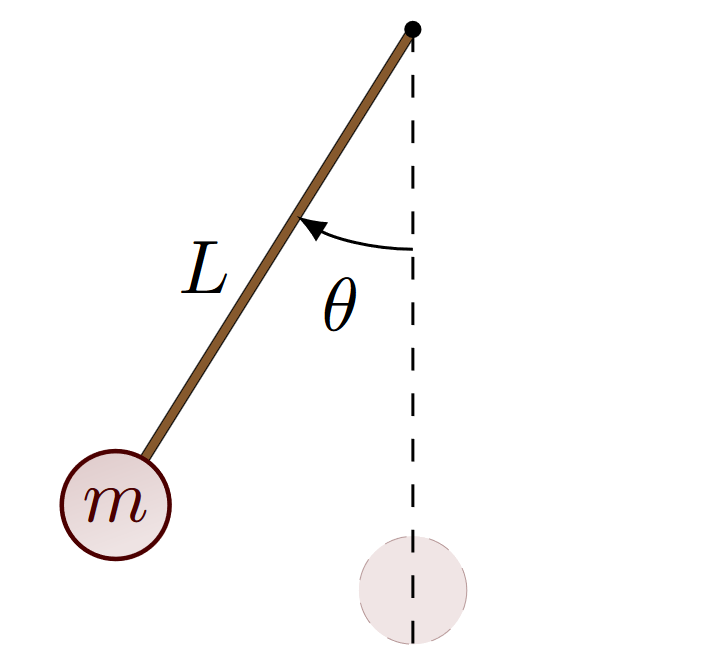
\includegraphics[width=0.7\linewidth]{pendulum.png}
    %\caption{Enter Caption}
    %\label{fig:enter-label}
\end{figure}

\vfill\null
\columnbreak

A pendulum is released with an initial angle $\theta_0$. As it swings, the period, $T$, is given by the following:
\pause
\[T(\theta_0)=2\sqrt{2}\sqrt{\frac{L}{g}}\int_0^{\theta_0} \frac{d\theta}{\sqrt{cos \theta - cos \theta_0}}\]

where $L$ is the length of the pendulum and $g$ is the gravitational constant.
\pause
\\
\\
\textbf{There is no closed-form anti-derivative for this integral!}
\end{multicols}
\end{frame}

\begin{frame}{Numerical Methods for Integration}
\begin{itemize}
\item Gaussian Quadrature
\item Romberg Algorithm
\item Simpson's Rule
\item \textbf{Trapezoid Rule}
\end{itemize}
\end{frame}

\begin{frame}{Approximation of Numerical Integration}
	General Approach
	\begin{enumerate}
		\item Use a simple function to approximate the integral area.
		\item Divide an integral into small segments.
	\end{enumerate}

	\begin{tikzpicture}[line join=round,line cap=round]
		\begin{scope}
		\draw[-latex] (-0.5,0) -- (10,0) node[below] {$x$};
		\draw[-latex] (0,-0.5) -- (0,4) node[left]  {$y$};
		\foreach\i in {0,1,2,3,4}
		{
			\pgfmathsetmacro\j{0.9*\i+0.9}
			\coordinate (x\i) at (\j * 2,0);
			\coordinate (y\i) at (\j * 2,{f(\j)});
			\pgfmathtruncatemacro\j{\i+1}
			\node[below]      at (x\i) {\j};
		}
		\foreach\i in {0,1,2,3,4}
		{
			\pgfmathtruncatemacro\j{\i+1}
			\ifnum\i<4
				\pgfmathsetmacro\x{0.9*\i+0.9}
				\filldraw[osprey_green] (\x*2, 0) rectangle ++(1.8, {f(\j) - 0.1});
				\draw[gray] (\x*2, 0) rectangle ++(1.8, {f(\j) - 0.1});
			\fi
		}
		\draw[thick,cyan] plot[domain=0.5:4.5,samples=41] (\x * 2,{f(\x)});
		\end{scope}
	\end{tikzpicture} \\
	\footnotesize \textit{Note:} Approximation is not vary accurate.
\end{frame}

\section{Trapezoid Rule}
\begin{frame}{Trapezoid Rule: Formula}
\[ \int_a^b f(x)dx \approx \frac{h}{2} (f(x_0) + f(x_n)) + \sum_{i=1}^{n-1} f(x_i) \]
where $h = (b-a)/n, x_i = a + ih$

Given p processes, each process can work on n/p intervals

Note: for simplicity will assume $n/p$ is an integer

\begingroup
\renewcommand{\arraystretch}{1.5}
\begin{center}
\begin{tabular}{ l l }
 \hline
 process & interval \\ 
 \hline
 0 & $[a, a + \frac{n}{p}h]$ \\ 
 1 & $[a + \frac{n}{p}h, a + 2\frac{n}{p}h]$ \\ 
 ... & ... \\  
 $p-1$ & $[a + (p - 1)\frac{n}{p}h, b]$ \\
 \hline
\end{tabular}
\end{center}
\endgroup

\end{frame}

\begin{frame}{Trapezoid Rule: Integration}
	\begin{multicols}{2}
	Area $ = \frac{1}{2}[f(a) + f(b)](b-a)$ \\
	
	\begin{spacing}{1.25}
		Area $ = \frac{1}{2}[f(x_0) + f(x_1)](x_1-x_0) +$ \\
		\phantom{x}\hspace{2.5em} $ \frac{1}{2}[f(x_1) + f(x_2)](x_2-x_1) +$
		\phantom{x}\hspace{2.5em} $ \frac{1}{2}[f(x_2) + f(x_3)](x_3-x_2) +$ \\

		\hspace{2em} $ = \frac{h}{2}[f(x_0) + f(x_1) +$ \\
		\phantom{x}\hspace{3.5em} $f(x_1) + f(x_2) + $ \\
		\phantom{x}\hspace{3.5em} $f(x_2) + f(x_3)]$
	\end{spacing}

	\begin{tikzpicture}[line join=round,line cap=round]
		\begin{scope}
		\draw[-latex] (-0.5,0) -- (5,0) node[below] {$x$};
		\draw[-latex] (0,-0.5) -- (0,5) node[left]  {$y$};
		\node at (3.25,3.5) {$y=f(x)$};
		\foreach\i in {0,1,2,3}
		{
			\pgfmathsetmacro\j{1*\i+1}
			\coordinate (x\i) at (\j,0);
			\coordinate (y\i) at (\j,{f(\j)});
			\node[below]        at (x\i) {$x_\i$};
		}
		\node[yshift=-0.75cm] at (x0) {\strut$a$};
		\node[yshift=-0.75cm] at (x3) {\strut$b$};
		\end{scope}
		\foreach\i in {0,1,2,3}
		{
			\pgfmathtruncatemacro\j{\i+1}
			\ifnum\i<3
				\filldraw[osprey_green] (x\i) -- (y\i) -- (y\j) -- (x\j);
				\draw[gray] (x\i) -- (y\i) -- (y\j) -- (x\j);
			\fi
			\fill (y\i) circle (1pt);
		}
		\draw[thick,cyan] plot[domain=0.5:4.5,samples=41] (\x,{f(\x)});
	\end{tikzpicture}
	\end{multicols}
	\vspace{-2em}
	\hspace{2em} $ = \frac{h}{2}[f(x_0) + 2f(x_1) + 2f(x_2) + f(x_3)]$
\end{frame}

\begin{frame}{Trapezoid Rule: Integration Error}
\animategraphics[autoplay,loop,width=\linewidth - 0.5cm]{1}{assets/Trapezium2-}{0}{19}
\end{frame}

\begin{frame}{Trapezoid Rule: Integration Accuracy}
	\begin{multicols}{2}
	Accuracy can be increased through increasing the number of partitions. \\
	
	The more trapeziums the area is divided into the more accurate the estimate. \\
	
	Error in approximation decreases as the partition step size decreases. \\

	Accuracy is reliant on increasing precision. \\

	Partition area calculations are independent.

	\begin{tikzpicture}[line join=round,line cap=round]
		\begin{scope}
		\draw[-latex] (-0.5,0) -- (5,0) node[below] {$x$};
		\draw[-latex] (0,-0.5) -- (0,5) node[left]  {$y$};
		\node at (3.25,3.5) {$y=f(x)$};
		\foreach\i in {0,1,2,3,...,8}
		{
			\pgfmathsetmacro\j{0.5*\i+0.5}
			\coordinate (x\i) at (\j,0);
			\coordinate (y\i) at (\j,{f(\j)});
		}
		\foreach\i in {0,1,2,3}
			\node[below]          at (x\i) {$x_\i$};
		\node[below]          at (x7) {$x_{n-1}$};
		\node[below]          at (x8) {$x_n$};
		\node[yshift=-0.75cm] at (x0) {\strut$a$};
		\node[yshift=-0.75cm] at (x8) {\strut$b$};
		\end{scope}
		\foreach\i in {0,1,2,3,...,8}
		{
			\pgfmathtruncatemacro\j{\i+1}
			\ifnum\i<8
				\filldraw[osprey_green] (x\i) -- (y\i) -- (y\j) -- (x\j);
				\draw[gray] (x\i) -- (y\i) -- (y\j) -- (x\j);
			\fi
			\fill (y\i) circle (1pt);
		}
		\draw[thick,cyan] plot[domain=0.5:4.5,samples=41] (\x,{f(\x)});
	\end{tikzpicture} \\
	\vfill
	\end{multicols}
\end{frame}

\begin{frame}{Trapezoid Rule: Accuracy}
	\begin{itemize}
		\item Numerical methods of integration, such as using the Trapezoid Rule, only provide an estimate of the actual area.
		\item More partitions/sub-intervals may lead to greater accuracy.
		\item How many partitions are needed to achieve a desired accuracy?
		\item There's a way to find out ahead of time!
		\item Unfortunately, we need to find the second derivative of the function being integrated, and we must do some analysis on that.
	\end{itemize}
\end{frame}

\begin{frame}{Trapezoid Rule: Accuracy}
	\begin{itemize}
		\item Suppose $E_T$ is the difference between our estimate and the exact value of the integral (which we don't have to know).
		\item This is the \textbf{Total Error} $E_T$.
		\item The following gives an upper bound for $|E_T|$ when integrating $f(x)$ on the interval $[a,b]$:
		\[|E_T|\leq(b-a)\frac{h^2}{12}M\]
		where $h$ is the partitions width,\\
		and $M$ is the maximum value of $|f''(x)|$ on the interval $[a,b]$.
		\item We specify a maximum bound for $|E_T|$, so after we determine $M$, we can solve for $h$ and subsequently solve for $n$, the number of partitions we need for our desired accuracy.
	\end{itemize}
\end{frame}

\begin{frame}[allowframebreaks]{Example: Calculate Number of Partitions}
Suppose we want to integrate
\[f(x)=\frac{100}{x+5}\]
on the interval $[0,100]$ using the Trapezoid Rule with a total error of no more than $10^{-4}$. So,
\[f''(x)=\frac{200}{(x+5)^3}\]
and on the interval $[0,100]$, $|f''(x)|$ is highest when $x=0$. So
\[M=\left|\frac{200}{5^3}\right|=1.6\]

\framebreak

Using the formula from a previous slide, we want to find $h$ (the partition width) such that

\[(b-a)\frac{h^2}{12}M\leq10^{-4}\]
which guarantees that the absolute value of the total error is also $\leq10^{-4}$.

Filling in the values we know for $b, a,$ and $M$ and then solve for $h$:

\[(100-0)\frac{h^2}{12}(1.6)\leq10^{-4}\]
\[h^2 \leq 0.0000075\]
\[h \leq 0.0027386\]

\framebreak

So the number of partitions/sub-intervals we need in order to find an answer to the integral within $10^{-4}$ of the exact answer is

\[n=\frac{b-a}{h}=\frac{100}{0.0027386}=36,515\]
\end{frame}

\section{Serial Implementation}
\begin{frame}{Serial Implementation: Approach}
	\begin{enumerate}
		\item Partition the interval $[a,b]$ into $n$ partitions/steps.
		\item Calculate the partition height $h$ based on $n$ steps. \\
			$h = \frac{(b-a)}{n}$
		\item Sum up each partition $n$ times.
	\end{enumerate}
\end{frame}

\begin{frame}[containsverbatim]{Serial Implementation: Code}
\begin{minted}{c}
/* Function being integrated using @$f(x) = x^2$@*/
float f(float x) {
	return x*x;
}
float trapezoid_rule(float a, float b, int n) {
	float result;
	float h;
	float x;
	int i;

	integral = (f(a) + f(b))/2.0;
	h = (b - a) / n;
	x = a;
	for ( i = 1; i <= n-1; i++ ) {
		x += h;
		result += f(x);
	}
	return result*h;
}
\end{minted}
\end{frame}

\section{Parallel Implementation}
\begin{frame}{Parallel Implementation: Approach}
	\begin{itemize}
		\item Split the interval $[a,b]$ up among the $p$ processes.
		\item Each process will estimate the integral $f(x)$ over its subinterval.
		\item To estimate the total integral, the processes’ local calculations are added.
		\item Suppose that the $n$ trapezoids are divided evenly across $p$ processes.
		\item Process $q$ will estimate the integral over the interval \\
		$[a + q\frac{nh}{p}, a + (q + 1)\frac{nh}{p}]$
		
		\item Each process needs the following information:
		\begin{itemize}
			\item Number of processes, $p$.
			\item Its rank.
			\item The entire interval of integration, $[a, b]$.
			\item The number of subintervals, $n$.
		\end{itemize}
	\end{itemize}
\end{frame}

\begin{frame}{Trapezoid Rule: Parallelizing}
	\begin{enumerate}
		\item Partition problem solution into tasks.
		\item Identify communication channels between tasks. (MPI)
		\item Aggregate tasks into composite tasks.
		\item Map composite tasks to cores.
	\end{enumerate}

	\begin{tikzpicture}[line join=round,line cap=round]
		\begin{scope}
		\draw[-latex] (-0.5,0) -- (10,0) node[below] {$x$};
		\draw[-latex] (0,-0.5) -- (0,4) node[left]  {$y$};
		\node at (6.5,3.5) {$y=f(x)$};
		\foreach\i in {0,1,2,3,4}
		{
			\pgfmathsetmacro\j{0.9*\i+0.9}
			\coordinate (x\i) at (\j * 2,0);
			\coordinate (y\i) at (\j * 2,{f(\j)});
			\node[below]       at (x\i) {$x_\i$};
		}
		\foreach\i in {0,1,2,3,4}
		{
			\pgfmathtruncatemacro\j{\i+1}
			\ifnum\i<4
				\filldraw[osprey_green] (x\i) -- (y\i) -- (y\j) -- (x\j);
				\draw[gray] (x\i) -- (y\i) -- (y\j) -- (x\j);
				\node at (\j * 1.75 + 1,2) {Task \i};
				\node at (\j * 1.75 + 1,1.5) {Core \i};
			\fi
			\fill (y\i) circle (1pt);
		}
		\draw[thick,cyan] plot[domain=0.5:4.5,samples=41,tension=1] (\x * 2,{f(\x)});
		\end{scope}
	\end{tikzpicture}
\end{frame}

\begin{frame}{Trapezoid Rule: Tasks \& Communication}
  \begin{tikzpicture}[node distance=3cm]
	\tikzset{
		->, % makes the edges directed
		>=stealth', % makes the arrow heads bold
		node distance=3cm, % minimum distance between two nodes. Change if necessary.
		every state/.style={thick, fill=gray!10}, % sets properties for each state node
		initial text=$ $, % sets the text that appears on the start arrow
	}
	\tikzstyle{bag} = [align=center]
    \node[state, draw=osprey_green, bag] (0) {Compute Area\\of Trapezoid 0};
    \node[state, right of=0, draw=osprey_green, bag] (1) {Compute Area\\of Trapezoid 1};
    \node[state, right of=1, draw=osprey_green, xshift=-2mm, bag] (2) {...};
    \node[state, right of=2, draw=osprey_green, xshift=-1mm, bag] (3) {Compute Area\\of Trapezoid\\$n-1$};
    \node[state, below of=1, draw=cyan, xshift=14mm, yshift=-10mm, bag] (4) {Add Areas};
    \draw[very thick]
      (0) edge[left, draw=black] node{} (4)
      (1) edge[left, draw=black] node{} (4)
      (2) edge[left, draw=black] node{} (4)
      (3) edge[left, draw=black] node{} (4);
  \end{tikzpicture}
\end{frame}

\begin{frame}[containsverbatim]{Parallel Implementation: Threaded Code}
\begin{minted}[fontsize=\scriptsize]{c}
// Calculate h and trapezoids per thread
double h = (b - a) / n;
int trapezoids_per_thread = n / num_threads;

// Create threads to compute trapezoidal rule in parallel
for (int i = 0; i < num_threads; i++) {
    thread_args[i].id = i;
    thread_args[i].local_a = a + i * trapezoids_per_thread * h;
    thread_args[i].local_b = thread_args[i].local_a +
                             trapezoids_per_thread * h;
    thread_args[i].local_n = trapezoids_per_thread;
    thread_args[i].f = es.equation_functions[f_idx];
    thread_args[i].mutex = &mutex;
    thread_args[i].global_sum = &global_sum;

    pthread_create(&threads[i], NULL, trapezoid_rule,
                   (void*)&thread_args[i]);
}

// Join threads
for (int i = 0; i < num_threads; i++) {
    pthread_join(threads[i], NULL);
}
\end{minted}
\end{frame}

\begin{frame}{Trapezoid Rule: Code Demos!}
\center
\Large\textbf{Let's Get Ready to Code!} \\ \, \\

\animategraphics[autoplay,loop]{50}{assets/keyboardpepe-}{0}{13}
\end{frame}

\begin{frame}{References}
\begin{itemize}
    \item Pendulum graphic: Licensed under a Creative Commons Attribution-ShareAlike 4.0 International License with Copyright 2021 – TikZ.net
    \item Pendulum formula: Kharab, A., \& Guenther, R. B. (2018). An introduction to numerical methods: A MATLAB Approach. Chapman \& Hall/CRC Numerical Analysis and Scientific Computing Series.
\end{itemize}
\end{frame}

\end{document}
